\documentclass[12pt]{report}
\usepackage[utf8]{inputenc}
\usepackage[T1]{fontenc}
\usepackage{german}
\usepackage{geometry}                % See geometry.pdf to learn the layout options. There are lots.
\geometry{a4paper}                   % ... or a4paper or a5paper or ... 
\usepackage[parfill]{parskip}    % Activate to begin paragraphs with an empty line rather than an indent
\usepackage{xifthen}
\usepackage{xstring}			% to check content of strings in xifthen
\usepackage{graphicx}
\usepackage[usenames,dvipsnames,table]{xcolor}
\usepackage{amssymb}
\usepackage{epstopdf}
\usepackage{hyperref}
\usepackage{fancyhdr}


\IfStrEq*{\languagename}{english}
	{
		\newcommand{\dalabel}{Diploma Thesis}
		\newcommand{\submittedlabel}{Submitted by}
		\newcommand{\datelabel}{Date}
		\newcommand{\supervisorlabel}{Supervisor}
		\newcommand{\projectpartnerlabel}{Project Partner}
	}
	{
		\newcommand{\dalabel}{Diplomarbeit}
		\newcommand{\submittedlabel}{Eingereicht von}
		\newcommand{\datelabel}{Datum}
		\newcommand{\supervisorlabel}{Betreuer}
		\newcommand{\projectpartnerlabel}{Projektpartner}
	}
 % This file should not really be touched
\newcommand{\titleofthesis}{HomeDS}
\newcommand{\department}{Informatik} % Replace by your department

\newcommand{\firstauthor}{Andrej Sakal}
\newcommand{\firstauthorclass}{5CHIF}
\newcommand{\secondauthor}{Felix Hofmann}
\newcommand{\secondauthorclass}{5CHIF}

\newcommand{\duedateen}{April 4, 2018} % due date in english format
\newcommand{\duedatede}{4. April 2018} % due date in german format
\newcommand{\supervisor}{Thomas Stütz}

 % Set basic data (author, title, etc.) of your thesis
\begin{document}
\rhead{\includegraphics[scale=.9]{images/Logo.png}}
\cfoot{}
\begin{titlepage}
\thispagestyle{fancy}

\begin{center}

\vspace*{8em}

{\LARGE \dalabel}

\vspace{2em}

{\large Höhere Technische Bundeslehranstalt Leonding \\[.5em]
Abteilung für \department}

%\vspace{8em}
\vspace*{\fill}

{\Huge \titleofthesis}
\end{center}

%\vspace{8em}
\vspace*{\fill}

\begin{tabular}{ll}
\ifthenelse{\isundefined{\firstauthor}}{}{\submittedlabel: & {\bf \firstauthor, \firstauthorclass}}
\ifthenelse{\isundefined{\secondauthor}}{}{ \\[.5em] & {\bf \secondauthor, \secondauthorclass}}
\ifthenelse{\isundefined{\thirdauthor}}{}{ \\[.5em] & {\bf \thirdauthor, \thirdauthorclass}}
\ifthenelse{\isundefined{\fourthauthor}}{}{ \\[.5em] & {\bf \fourthauthor, \fourthauthorclass}}
 \\[.5em]
\datelabel: & {\bf \duedateen} \\[.5em]

\supervisorlabel: & {\bf \supervisor} \\[.5em]

\ifthenelse{\isundefined{\projectpartner}}{}{\projectpartnerlabel: & {\bf \projectpartner}}
\end{tabular}
\end{titlepage}
 % Should not be necessary to touch this file
\section*{Declaration of Academic Honesty}
Hereby, I declare that I have composed the presented paper independently on my own and without any other resources than the ones indicated. All thoughts taken directly or indirectly from external sources are properly denoted as such.

This paper has neither been previously submitted to another authority nor has it been published yet. \\[1em]
Leonding, \duedateen \\[5em]
\ifthenelse{\isundefined{\firstauthor}}{}{\firstauthor}
\ifthenelse{\isundefined{\secondauthor}}{}{\kern-1ex, \secondauthor}
\ifthenelse{\isundefined{\thirdauthor}}{}{\kern-1ex, \thirdauthor}
\ifthenelse{\isundefined{\fourthauthor}}{}{\kern-1ex, \fourthauthor} \\[5em]

\begin{otherlanguage}{german}
\section*{Eidesstattliche Erkl�rung}
Hiermit erkl�re ich an Eides statt, dass ich die vorgelegte Diplomarbeit selbstst�ndig und ohne Benutzung anderer als der angegebenen Hilfsmittel angefertigt habe. Gedanken, die aus fremden Quellen direkt oder indirekt �bernommen wurden, sind als solche gekennzeichnet.

Die Arbeit wurde bisher in gleicher oder �hnlicher Weise keiner anderen Pr�fungsbeh�rde vorgelegt und auch noch nicht ver�ffentlicht. \\[1em]
Leonding, am \duedatede \\[5em]
\ifthenelse{\isundefined{\firstauthor}}{}{\firstauthor}
\ifthenelse{\isundefined{\secondauthor}}{}{\kern-1ex, \secondauthor}
\ifthenelse{\isundefined{\thirdauthor}}{}{\kern-1ex, \thirdauthor}
\ifthenelse{\isundefined{\fourthauthor}}{}{\kern-1ex, \fourthauthor} \\[5em]
\end{otherlanguage}

\begin{abstract}
Die HTL-Leonding besitzt schon einige Multimedia Systeme verstreut im ganzen Schulgeb�ude um Projekte, aktuelle News und �nderungen im Unterrichtsablauf anzuzeigen. Doch ein gro�er Schwachpunkt dieser Multimedia Systeme ist, dass der Prozess vom erstellen der Anzeige bis zum zuordnen welcher Bildschirm, welche Information anzeigen soll sehr kompliziert, und m�hselig ist. Sodass oftmals neue Informationen erst Versp�tet oder gar nicht angezeigt wird.

Unsere Diplomarbeit besch�ftigt sich mit dem erschaffen eines gemeinsames System zu entwickeln um einfach neue Supplierungen, Nachrichten oder Eilmeldungen auf allen Bildschirmen der HTL-Leonding anzuzeigen. Diese Systeme werden unter dem Begriff "Digital Signage System" zusammengefasst.


 % Declaration of Academic Honesty, Abstracts, Acknowledgments, 

\tableofcontents

\chapter{Einleitung}
\section{Ausgangssituation}
Die HTL-Leonding besitzt schon einige Multimedia Systeme verstreut im ganzen Schulgeb�ude um Projekte, aktuelle News und �nderungen im Unterrichtsablauf anzuzeigen. Doch ein gro�er Schwachpunkt dieser Multimedia Systeme ist, dass der Prozess vom erstellen der Anzeige bis zum zuordnen welcher Bildschirm, welche Information anzeigen soll sehr kompliziert, und m�hselig ist. Sodass oftmals neue Informationen erst Versp�tet oder gar nicht angezeigt wird. 

\section{Ziele}
Die Ziele sind das die HTL Leonding den Sch�lern schneller Information oder Eilmeldungen auf den Multimedia System anzuzeigen.

\section{Overview}
Details of the diploma thesis have to be aligned between student and supervisor. This should be a basic structure to facilitate the first steps when students start to write their theses.

Never forget to add some illustrative images. Images must not be messed up with your normal text. They are encapsulated in floating bodies and referenced in your text. An example can be seen in figure~\ref{fig:sample}. As you can see, figures are placed by default on top of the page nearby the place where they are referenced the first time. Furthermore you can see that a list of figures is maintained automatically which can be included easily by typing the command \verb1\listoffigures1 into your document.

\begin{figure}
\begin{center}
	\includegraphics[scale=.5]{images/don_knuth.jpg}
\end{center}
	\caption{Don Knuth, the inventor of \TeX}
	\label{fig:sample}
\end{figure}

\section{Basic Terminology}
As usual the very basic terminology is briefly explained here. Most probably the explanations here only scratch a surface level. More detailed explanations of terminology goes into chapter~\ref{cha:theoretical-background}.

\section{Related Work and Projects}
Here a survey of other work in and around the area of the thesis is given. The reader shall see that the authors of the thesis know their field well and understand the developments there. Furthermore here is a good place to show what relevance the thesis in its field has.

\section{Structure of the Thesis}
%dsflkjas flaksjfl asdfj as lfjldsajflaksdjf sa dfjlasdkfj sadlfjasdklf als dfj l dfsdfsdfn chapter~\ref{cha:used-technologies} (\nameref{cha:used-technologies}) on page~\pageref{cha:used-technologies} we describe the used technologies.
Finally the reader is given a brief description what (s)he can expect in the thesis. Each chapter is introduced with a paragraph roughly describing its content.
\chapter{Digital Signage \& XIBO}
\section{Was ist Digital Signage?}\label{sec:digitalsignage}
Digital Signage, in Deutsch Digitales Schild, hat grundsätzlich die Aufgabe Inhalte die meist auf Plakaten oder Schildern angezeigt werden auf Bildschirmen anzuzeigen. Mithilfe von Digital Signage Systemen, soll das zeit- oder interaktionsgesteuerte Ändern von Inhalten auf den Bildschirmen einfach und übersichtlich gehalten werden siehe Abbildung \ref{img:digitalsignagehtlleonding}. Weiteres bietet Digital Signage ein breites Spektrum an Anwendungsbereichen. Digital Signage ist vor allem im Marketing Bereich ein sehr beliebtes Mittel, um ein neues Produkt oder eine Neuheit zu präsentieren. 

https://de.wikipedia.org/wiki/Digital_Signage#Anwendungsbeispiele:_2017.


\begin{figure}[H]
\centering
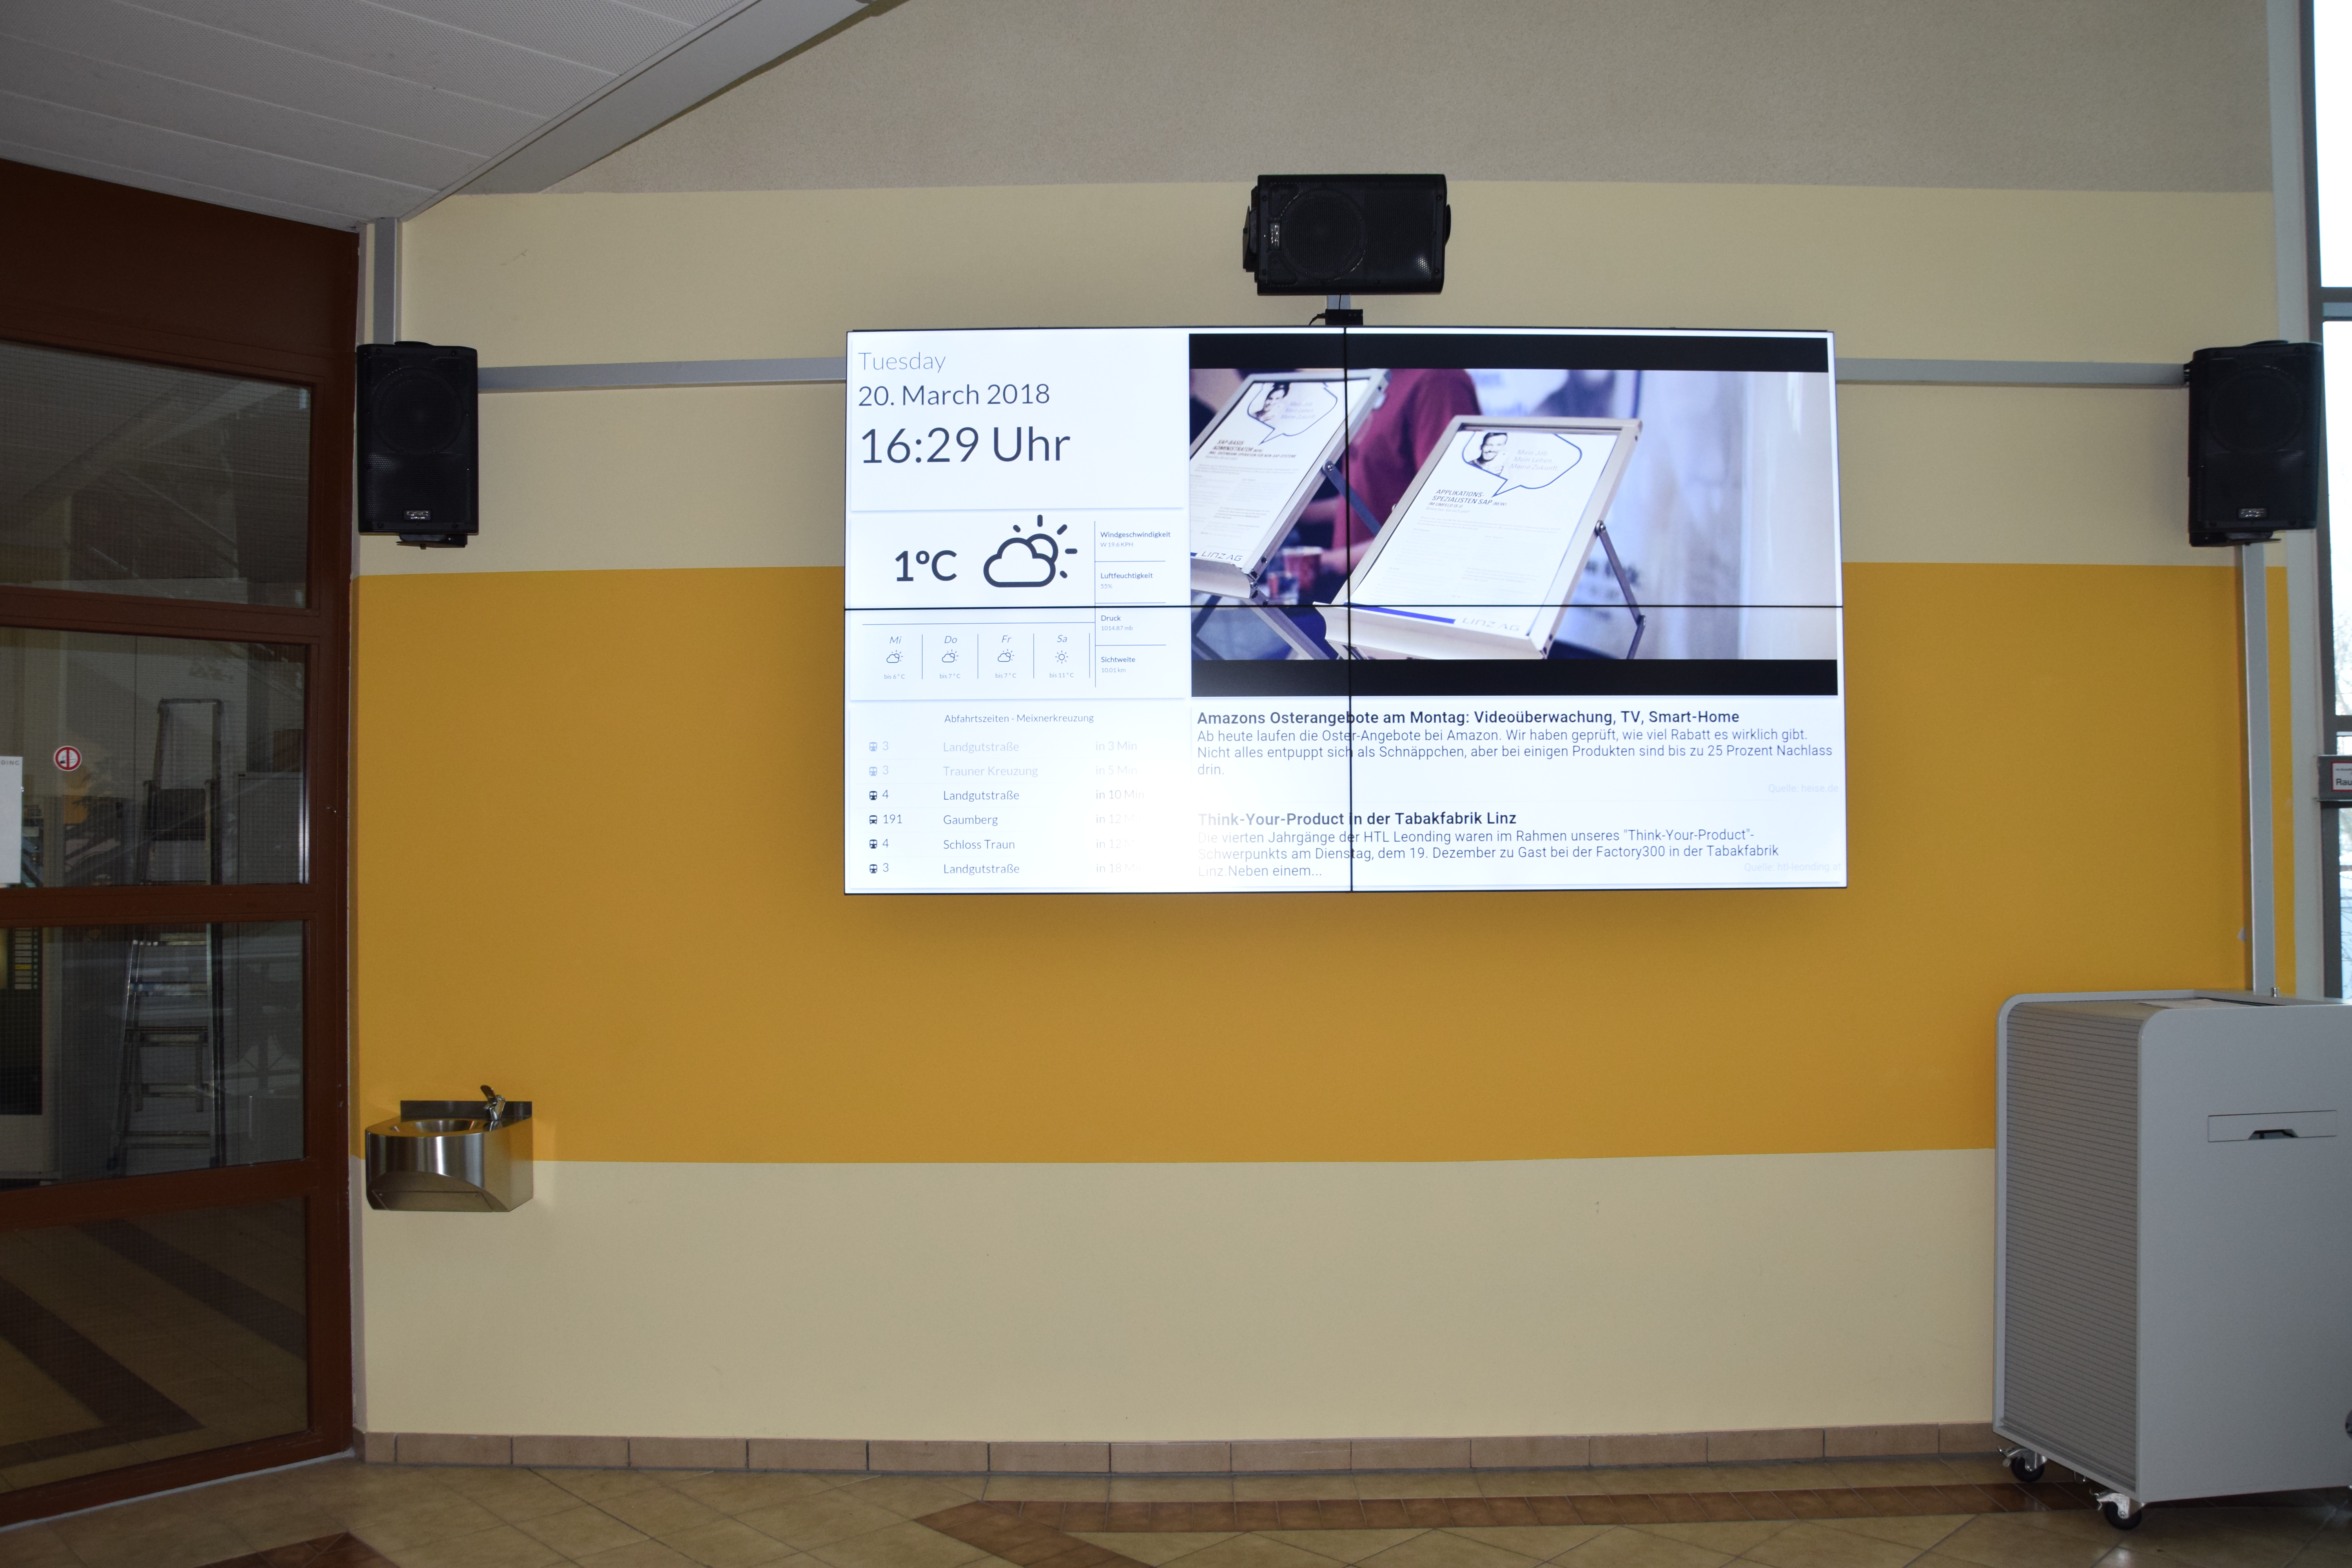
\includegraphics[width=1\textwidth]{images/02_XiboGrundlagen/Videowall.JPG}
\caption{Digital Signage in der HTL Leonding}
\label{img:digitalsignagehtlleonding}
\end{figure}

\section{Digital Signage Anwendungen}\label{sec:anwendungedigitalsignage}
Digital Signage hat keine Grenzen und kann vielfältig eingesetzt werden. Viele Konzerne nutzen Digital Signage für Marketing Zwecke, Produkte zu präsentieren oder oft auch nur als Lockmittel.

\section{Was ist XIBO?}\label{sec:xibo}
Das XIBO ist ein Open Source Digital Signage System entwickelt von der Spring Signage LTD. Das XIBO-System besteht aus vielen verschiedenen Komponenten. Das XIBO Paket besteht aus einem klassischen Server-Client Konstrukt. Der Server besteht aus drei Komponenten: das Content Managment System welches mithilfe von ZeroMq bei Änderung der Inhalte diese aktualisieren soll, einer Datenbank und einer Weboberfläche, die es dem Benutzer ermöglichen soll das System zu bedienen.

\section{Weboberfläche des XIBO}\label{sec:webpagexibo}
Das Steuerungszentrum des ganzen Signage System ist die Weboberfläche, die ganz einfach über einen Browser unter der Serveraddresse aufgerufen werden kann. Auf der Willkommensseite sind die wichtigsten Funktionen des Signage Servers dargestellt:

\begin{enumerate}
	\item {\em Kalender:} Mit der Kalender Funktion kann eingetragen werden zu welchem Zeitpunkt, welcher Inhalt, auf welchem Bildschirm angezeigt werden soll. Diese Funktion ist einer der wichtigsten und meist verwendeten. In dem Xibo-Kalender werden auch bereits eingetragene Aktivitäten angezeigt.

\begin{figur}
	\centering
\includegraphics[width=1\textwidth]{images/xibo-basics-calendar}
	\label{img:calendar}
	\caption{XBIO - Kalender}
\end{calendar}	
	
	\item {\em Layouts:} 
	Die Layout-Funktion ist einer der wichtigsten Komponenten des Signage Systems. Es beschäftigt sich mit dem Designen der Inhalte. Auf diese Funktion kommen wir noch einmal zurück.
	
	\item {\em Bibliothek:} 
	Die Bibliothek-Funktion ist zuständig für das Verwalten der Medien. Hier können Sie verschiedene Dateien hochladen.  Diese Medien können dann in Layouts eingebunden und angezeigt werden.
	
	\item {\em Benutzer:} 
	Im Menüpunkt Benutzer können neue Benutzer angelegt und bereits bestehende bearbeitet oder gelöscht werden. Dabei gibt es auch ein Rechte-System. Es können auch Datenmengenbegrenzungen pro Benutzer eingestellt werden.
	
	\item {\em Einstellungen:} 
	Der Menüpunkt Einstellungen gibt dem Nutzer die Möglichkeit, verschiedene Optionen zu wählen. So sind zum Beispiel die richtige Zeitzone, E-Mail Benachrichtigungen, wichtige Einstellungen, die für ein einwandfreies Funktionieren des Xibo-Servers zuständig sind. Aus den Einstellungen ist auch der CMS geheimer Schlüssel zu finden, der für die Authentifizierung der API Zugriffe zuständig ist herauszulesen.
\end{enumerate}

\section{Designen mit XIBO}\label{sec:designexibo}
Beim Designen von einem neuen Layout im XIBO, muss zuerst die Bildschirmauflösung ausgewählt und dem Layout ein passender Name zugewiesen werden, sowie optional auch eine Beschreibung. 

\textbf{Layout Maske}

\begin{calendar}
	\centering
\includegraphics[width=1\textwidth]{images/xibo-basics-designer}
	\label{img:designeLayout}
	\caption{XIBO-Layout designen}
\end{calendar}	

Dem Layout kann nun eine Region oder auch mehrere  hinzugefügt werden. Eine Region kann mehrere Widgets enthalten. Mit einem Doppelklick auf die Region kann ein Widget hinzugefügt werden. Es gibt viele verschiedene Arten von Widgets:

\begin{widgettypes}
	\item {\em Bibliothek:} Mit diesem Widget können Elemente aus der Medienbibliothek in der Region angezeigt werden. Dabei werden PowerPoint Formate, Video, Bilder und andere Medien Datentypen unterstützt.
	
	\item {\em Uhr:} 
	Dieser Widgettyp bindet eine Uhr in die Region ein. Es kann entweder eine Uhr im Analogen Stil oder Digitalen Stil ausgewählt werden.
	
	\item {\em DataSet:} 
	Das DataSet Widget ist sehr wichtig und zeigt grob gesagt nacheinander Daten aus einem Array mit Key, Value Paaren an.
	
	\item {\em Wheather:} 
	Das Wheather Widget, in Deutsch Wetter, zeigt das aktuelle Wetter an. Es kann eingestellt werden ob es anhand von den GPS-Daten des Bildschirmes die Wetterdaten anzeigen soll oder ein vorher definierter Ort für die Daten verwendet werden soll.
	
	\item {\em Flash:} 
	Mit dem Flash Widget können Flash Inhalte abgespielt werden.
	
	\item {\em HLS:} 
	Mit dem HLS Widget können HLS Video Streams angezeigt werden.
	
	\item {\em Image:} 
	Mit dem Image Widget können Bilder entweder aus der XIBO Bibliothek angezeigt oder neue hochgeladen werden.
	
	\item {\em Local Video:} 
	Mit dem Local Video Widget können Videos oder Streams angezeigt werden.
	
	\item {\em PDF:} 
	Mit dem PDF Widget können PDFs entweder aus der XIBO Bibliothek angezeigt oder neue hochgeladen werden.
	
	\item {\em PowerPoint:} 
	Mit dem PowerPoint Widget können PowerPoint Präsentationen entweder aus der XIBO Bibliothek angezeigt oder neue hochgeladen werden.

	\item {\em Text:} 
	Mit dem Text Widget können Texte angezeigt werden.
	
	\item {\em Ticker:} 
	Mit dem Ticker Widget können Texte animiert angezeigt werden. Dabei können diese Texte aus einem DataSet oder einem RSS Feed stammen.
	
	\item {\em Webpage:} 
	Mit dem Webpage Widget können Webseiten angezeigt werden.
\end{widgettypes}

Nachdem eines der Widgets erstellt wurde kann das Ergebnis des Layouts mit einer Layout Vorschau kurz überprüft werden.

\chapter{XIBO-Server}
\section{Beschreibung}
Als zentrale Steuereinheit wird ein XIBO-Server verwendet. Um diesen verwenden zu können, war es notwendig sich in die Dokumentation einzulesen und die API-Schnittstelle auszuprobieren. Die Website des Servers diente vorerst als Übungsumgebung. Dadurch wurde es leicht auch die einzelnen Funktionen, inklusive der Vorgangsweise, des Servers zu verstehen.
\cite{xibo-server}
\section{API-Schnittstelle}
Die API-Schnittstelle des XIBO-Servers ist mittels Swagger dokumentiert. Diese Dokumentation deckt die Grundfunktionalitäten und die Form der Anfragen ab. Da die Schnittstelle des Servers später als wesentliches Verbindungsstück zwischen der eigens entwickelten Steuerungssoftware und dem Server dient, war es nötig, diese gründlich zu testen und auch zu verstehen. Anfangs wurde dafür mit Postman gearbeitet. Um mit Postman die Requests testen zu können musste festgestellt werden, welche Codierung für den Request verwendet wird. Im Falle des XIBO-Servers wird ''application/x-www-form-urlencoded'' als Codierung verwendet. Die Anfragen an den Server wurden im Java Code durch die ''libary'' OkHttp3 übernommen.
\cite{swagger}
\cite{postman}
\cite{Okhttp3}
\section{Authentifizierung}
Bevor ein Client(im Zuge der Diplomarbeit handelt es sich um den Java-EE-Server) Anweisungen an den XIBO-Server in Form von Rest-Reqests übermitteln kann muss sich dieser mittels OAuth2 authentifizieren. Dazu benötigt der eine vom Server generierte Client\_ID.
\cite{oAuth2}

Die Parameter: 
\begin{itemize}
	\item {\em Client\_ID:} XIBO-Server Anwendungen neue Anwendung
	\item {\em Client\_Secret:}  XIBO-Server Anwendungen neue Anwendung
	\item{\em grant\_type:} Muss in der Form ''&grant\_type=client\_credentials''
\end{itemize}
müssen dem Server übermittelt werden um die Authentifizierung mit dem XIBO-Server durchzuführen. Dies geschieht unter der URL ''api\/authorize\/access\_token''.






HomeDS\HomeDsBackend\src\main\java\at\htl\utils\AuthentificationHandler.java

Zuerst wird ein Request-Body erstellt. Dieser hat folgende Parameter in der Form: 
 ''client\_id=<CLIENT\_ID>\&client\_secret=<CLIENT\_SECRET>\&grant\_type=
 client\_credentials''
, die im Body mitgegeben werden und als Format 'application/x-www-form-urlencoded'  haben. Anschließend werden dem Header noch der "content-type'' mit dem Wert ''application/x-www-form-urlencoded'' und der Parameter ''cache-control'' mit dem Wert ''no-cache'' hinzugefügt. Als Ergebniss der Anfrage bekommt der Client einen '' access\_token '', dieser ist nun bei jeder Anfrage notwendig um sich beim Server zu authentifizieren und es dem Client zu ermöglichen Daten abzurufen beziehungsweise weiterzugeben.





\chapter{Verwendete Technologien}
\section{Git und GitHub}
Um als Team dynamisch arbeiten zu können, verwenden wir Software zur Versionsverwaltung. Hierbei handelt es sich um Git. 
Github ist die verwendete Online-Plattform, auf der Benutzer ihre Projekte gratis als Repository speichern. Dies ermöglicht einfaches arbeiten im Team und verhindert in den meisten Fällen Zusammenführungskonflikte. Mittels Git lässt sich auch einfach zurückverfolgen welches Teammitglied welche Änderungen gemacht hat. Bei Bedarf ist es möglich diese Änderungen zurückzusetzen.

Verwendet wird GitHub für die gesamte Diplomarbeit, sowohl für die Versionsverwaltung der Dokumente, als auch die einzelnen Applicationen. Um sicherzustellen, dass keine Konflikte durch paralleles Arbeiten entstehen, wird in Branches gearbeitet. Diese Branches wurden erstellt, wenn ein neues Arbeitspaket begonnen wurde, zum Beispiel die Android-App.

Bild Github und verweis Git/GitHub

\section{Android}

Android ist ein Betriebssystem für mobile Endgeräte, spezialisiert auf Touch-Anwendungen. Ziel ist es das Endgerät möglichst intuitiv und flexibel bedienen zu können. Mit Android ist es möglich open-source Applicationen zu erstellen, welche ein großes Publikum erreichen. Google stellt hier seinen eigenen ''PlayStore'' zur Verfügung, in dem die Applikationen gratis oder auch gegen Entgelt erworben werden können.
Diese Aspekte open-source, frei erhältlich und das Erreichen großes Publikum, sind ausschlaggebend dafür, dass die Applicationen in Android implementiert wird. Als Programmiersprache wird Java verwendet.
\\
\section{Java Enterprise Edition}\label{sec:javaee}
Die Java Platform, Enterprise Edition oder abgekürzt auch Java EE ist die technische nähere Beschreibung einer Softwarearchitektur, die programmierte Java Anwendungen ausführt.
(weiter ausführen)

QUELLE: https://de.Wikipedia.org/wiki/Java_Platform,_Enterprise_Edition

\section{JSF - Java Server Faces}\label{sec:javaee}
JSF ist ein Java Enterprise Edition Framework, welches zur Entwicklung von Webanwendungen verwendet wird. JSF wurde als Nachfolger von JSP eingeführt um die Mischung von HTML Code und Java Code übersichtlicher zu gestalten. Ziel der JSF Vorgehensweise ist es Anwendungen in Komponenten zu teilen, welche im besten Fall wiederverwendbar sind.

\section{IntelliJ IDEA}
Herausgeber dieser Entwicklungsumgebung ist JetBrains. Durch diese IDE wird die Entwicklung des Java-EE-Backends unterstützt, wobei Java nicht die einzige Programmiersprache ist, die in IntelliJ verwendet werden kann. Andere Programmiersprachen, wie zum Beispiel Groovy und Kotlin, können in der IDE ebenfalls programmiert werden. Des weiteren gibt es eine Vielzahl an Tools wie zum Beispiel der direkte Zugang zu diversen Datenbanken, beispielsweise wie MySQL Datenbanken, oder die Integration von ''build automation tools'' wie bower oder grunt. Zudem sind verschiedenste Versionsverwaltungssysteme wie GutHub mit IntelliJ kompatibel und ebenfalls direkt über die Benutzeroberfläche der IDE verwendbar.

\section{Android Studio}
Android Studio ist eine von Google und JetBrains bereitgestellte integrierte Entwicklungsumgebung um Android Applikationen zu entwickeln. Grundgerüst für die Entwicklungsumgebung, ist die ''IntelliJ IDEA''. Zu dem können über Android Studio Emulatoren verschiedenster Android Geräte heruntergeladen und gestartet werden, damit erstellte Applikationen leicht zu probieren sind. Zusätzlich bietet Android Studio GitHub Integration und einen großen Umfang an Werkzeugen und Testmöglichkeiten.
  
\chapter{HomeDS - Server}
\section{Einleitung}\label{sec:einleitung}
Im Rahmen der Diplomarbeit wird neben dem XIBO-Server ein eigen Programmierter Java Enterprise Edition Server eingesetzt. Aufgrund der hohen Komplexität des Signage-Servers aber relativ dünn dokumentierten API-Schnittstellen und begrenzten technischen Möglichkeiten muss ein eigen programmierter Server eingesetzt werden. Dieser wird die Kommunikation vom Signage Server zur Android App erleichtern.  
 
\section{Java Enterprise Edition}\label{sec:javaee}
Java Platform, Enterprise Edition, oder abgekürzt auch Java EE ist die technische nähere Beschreibung einer Softwarearchitektur die Java Programmierte Anwendungen ausführt.
(weiter ausführen)

QUELLE: https://de.Wikipedia.org/wiki/Java_Platform,_Enterprise_Edition
 
\section{Anforderungen an den HomeDS Server}\label{sec:homeds}
Der JavaEE Server soll die verschiedenen komplizierten Abläufe des XIBO-Servers vereinfachen. Die verschiedenen Zugriffe mittels REST die eigentlich direkt auf den XIBO laufen sollen werden über den JavaEE Server verwaltet. Dies hat insofern Vorteile da die komplizierten und meist mit viel Aufwand verknüpften Authentifizierungen wegfallen. Somit können ohne Probleme neue Funktionen hinzugefügt werden und ohne Probleme an neue Anforderungen angepasst werden.
 
\section{Funktionen des HomeDS Server}\label{sec:homedsfunction}
Der JavaEE Server verfügt über eine eigene MySQL Datenbank. Diese wird gebraucht um die "DataSets" aus dem Signage-Server zwischen zu speichern. Dies ist insofern erforderlich da die Aufgabenstellung erfordert die Datensätze entweder nur ab einem bestimmten Datum im Layout anzuzeigen oder bis zu einem bestimmten Datum diese angezeigt werden dürfen. 
 
\section{DataSet mit Ablaufdatum}\label{sec:datasetexpiredate}
Einer der wichtigsten Funktionen des Servers ist das hinzufügen, ändern und löschen vom DataSet. Da der Digital Signage Server über keine Felder wie Start- und Enddatum verfügen.

Die Logik ist simple der Benutzer kann Start- und Enddatum eingeben für jeden einzelnen DataSet eingeben. Und erst wenn das Datum genau in diesem Zeitintervall inklusive den Grenzen liegt wird das DataSet an den Xibo mittels API-Schnittstelle weitergegeben. 

\begin{lstlisting}
if (dataset.isActive() == false && (dataset.getFromDate().minusDays(1)
        .isBefore(LocalDate.now()))) {
    try {
        //if succesfull added then set active true and add id
        if ((id=dataSetApi.addDataSetField(dataset)) > 0) {
            dataset.setDataRowId(id);
            dataset.setActive(true);
            dataSetFieldFacade.save(dataset);
        }
    } catch (NoConnectionException e) {
        // Catch Exception
    }
}
\end{lstlisting}

Die Überprüfung ob die DataSets aus der Server-Datenbank im Zeitintervall liegen wird mittels eines "TimeSchedule" jeden Tag um 01:00 Uhr durchgeführt. Falls dieser dann im Intervall liegt wird der DataSet an den XIBO Signage Server gesendet. Diese Überprüfung beinhaltet auch das FromDate dies löscht bei überschreiten des Bis-Datums das DataSet aus dem Digital Signage heraus. 

Die Überprüfung ob das Startdatum heute oder vor dem heutigem Datum wird mithilfe der Java Annotation @Schedule realisiert. (siehe Codeausschnitt) 


 
\begin{enumerate}
  \item {\em :} Mit der Kalender Funktion kann eingetragen werden zu welchen Zeitpunkt welcher Inhalt auf welchem Bildschirm angezeigt werden soll. In dem Xibo-Kalender werden auch bereits eingetragene Aktivitäten angezeigt.
 
\begin{calendar}
  \centering
\includegraphics[width=1\textwidth]{images/xibo-basics-calendar}
  \label{Calendar}
\end{calendar}  
  
  \item {\em Layouts:} 
  Die Layout Funktion ist einer der wichtigsten Komponenten des Signage Systems es beschäftigt sich mit dem designen der Inhalte. Auf diese Funktion kommen wir noch einmal zurück
  
  \item {\em Bibliothek:} 
  Die Bibliothek Funktion ist zuständig für das Verwalten der Medien. Hier können Sie verschiedene Dateien hochladen.  Diese Medien können dann in Layouts eingebunden und angezeigt werden.
  
  \item {\em Benutzer:} 
  Im Menüpunkt Benutzer können neue Benutzer angelegt werden und bereits bestehende bearbeitet oder gelöscht werden. Dabei gibt es auch ein Rechte-System. Es könne auch Datenmengen Begrenzungen pro Benutzer eingestellt werden.
  
  \item {\em Einstellungen:} 
  Der Menöpunkt Einstellung gibt dem Nutzer die Möglichkeit verschiedene Optionen einzustellen. So sind zum Beispiel die richtige Zeitzone, E-Mail Benachrichtigungen wichtige Einstellungen die für ein Einwandfreies funktionieren des Xibo-Servers zuständig wichtig sind.
\end{enumerate}
 
\section{Designen mit XIBO}\label{sec:designexibo}
Beim Designen von einem neuen Layout im XIBO muss zuerst die Bildschirm auflösung ausgewählt werden. Und dem Layout ein passender Name zugewiesen werden sowie optional auch eine Beschreibung. 
 
\textbf{Layout Maske}
 
\begin{calendar}
  \centering
1 file change in working directory
View change
commit:c95ae5
WIP on master: Auto stash before merge of "master" and "origin/master"

\chapter{Android Application}
\section{Einleitung}
Um eine höchst mögliche Reichweite an Endgeräten zu erzielen, wurde eine Android Applikation entwickelt, mit der die wichtigsten Funktionen abgedeckt werden. Zum Beispiel das Wechseln der DataSets des Digital Signage Servers. Wichtig war es die Applikation möglichst einfach und leicht bedienbar zu gestalten, um auch Erstbenutzern die Bedienung zu erleichtern. 
Prototyp für die aktuelle Applikation war eine Anwendung für Android, die direkt mit dem Digital Signage Server kommuniziert, da sehr schnell klar wurde, dass das Steuern des Servers direkt über eine Applikation auf Android Basis viel zu umständlich ist. Es wurde eine weitere Mobile Applikation entwickelt, welche über das ''HomeDsBackend'' kommuniziert, um das Funktionsspektrum zu erweitern und die Applikation möglichst kompakt zu gestalten. Beispielsweise ist es durch diese Aufteilung nicht mehr nötig eine Datenbank in der Applikation zu haben. Somit erleichtert es auch Applikationen für andere Betriebssysteme zu implementieren. 


\section{Anforderungen}
Die Anforderungen an die Android Applikation weichen von den Anforderungen an das ''Backend'' leicht ab, da das ''Backend'' die gesamte Zeitsteuerung- und Datenbankfunktionalität übernimmt. Es besteht die Möglichkeit, den Server über die Website des ''Backend'' zu steuern, beziehungsweise über die Applikation auf Android Basis. 

\begin{itemize}
	\item {\em Eilmeldungen:} Dem Benutzer soll es möglich sein Nachrichten in einem Ticker auf den Bildschirmen anzuzeigen.
	
	\item {\em Medien Wiedergabe:} Medien die Lokal am Digital Signage Server liegen sollen abgespielt werden können.
		
	\item {\em Authentifizierung automatisieren (Prototyp Applikation):} Die Authentifizierung am Digital Signage Server soll automatisiert werden, um nicht vom Benutzer durchgeführt werden zu müssen.  
		
\end{itemize}

\section{Verwendete Technologien}
Android wird mit der API(Englisch: application programming interface / Deutsch: Anwendungsprogrammierschnittstelle), in der Version 26 (Oreo / Android 8.0) verwendet. 
VERWEIS ANDROID !!!!
Als Erweiterung für die Http Anfragen an den Digital Signage Server und das HomeDsBackend wird OkHttp3 verwendet.

\section{Struktur}
\begin{itemize}
	\item {\em activity:} Alle Activities die für die Anwendung benötigt werden. Als Beispiel die MainActivity
	
	\item {\em adapter:} Hier befinden sich alle Adapter für die RecyclerViews.
	
	\item {\em apiClient:} Beinhaltet die Klasse ''RequestHelper'' mit der die Anfragen an den Digital Signage Server beziehungsweise an das HomeDsBackend vereinfacht werden.
	
	\item {\em entity:} Jene Klassen die als Models für die Anwendung benötigt werden. 
	STÜTZ!!!
	
	\item {\em enumeration:} Enumerationen welche die Android Basierte Applikation verwendet. Zum Beispiel das ''RequestTypeEnum''.
	
	\item {\em fragment:} Alle Fragments die für das User Interface benötigt werden. Beispiel hierfür ist das Fragment ''NewsOverviewFragment'', welches alle DataSets die am Server sind anzeigt.
	
	\item {\em viewholder:} Beinhaltet alle ''ViewHolder'' die für die Verschiedenen ''RecyclerViews'' benötigt werden. 
	  
		
\end{itemize}

\section{MainBottomNavigationActivity und OverveiwFragment}
Die ''MainBottomNavigationActivity'' ist die Einzige ''Activity'' die in der Android Applikation benötigt wird. Hauptaufgabe der ''MainBottomNavigationActivity'' ist es, zwischen den einzelnen ''Fragments'' zu navigieren. Enthalten sind dazu jene Methoden, welche mit dem ''SupportFragmentManager'' die einzelnen Fragments im ''container\_main'' austauschen. Der ''container\_main'' ist ein ''ConstraintLayout'' welches in der zur ''MainActivity'' gehörenden Layout Ressource ''activity\_main.xml'' mit der Identifikationsnummer ''container\_main'' belegt wurde. Zudem wird die Klasse durch das Interface ''AppCompatActivity'' erweitert und implementiert die ''OnFragmentInteractionListener'' der Fragmente die in der Applikation verwendet werden. 


\title{onCreate}
Hier wird die ''Main\_Activity'' als ''ContentView'' gesetzt, zudem wird mittels ''SupportFragmentManager'' das ''HomeScreenFragment'' dem ''container\_main'' zugewiesen und angezeigt. Die statische Variable ''instance'', vom Datentyp ''MainActivity'', wird auf die aktuelle Instanz der Klasse zugewiesen. 
	
\title{getInstance}
 Ist der ''Getter'' für die statische Variable ''instance'' und übergibt die aktuelle Instanz der Klasse.
	
\title{''Fragment'' Austausch Methoden}
 Sind jene Methoden die für das Austauschen der einzelnen ''Fragments'' im ''container\_main'' zuständig sind. Dies geschieht mittels ''SupportFragmentManager'' welcher immer die ''Fragments'' im ''container\_main'' anzeigt und dem ''BackStack'', welcher für die Rückwerts Navigation (mittels retour Knopf des Mobilen Endgerätes) in der Applikation zuständig ist,  hinzufügt. Manche Methoden übergeben zudem noch ein ''Bundle'' an das erstellte ''Fragment'', welches Objekte enthält die in nächsten ''Fragment'' benötigt werden. Erkennungsmerkmal dieser Methoden ist das englische Verb ''open'' am beginn des Methodennamens. Als Namensbeispiel hierfür wird die Methode ''openNewsEditFragment'' herangezogen.





\section{DataSet verwaltung}
Die beiden Fragmente  ''NewsOverviewFragment'' und ''NewsEditFragment'' sind für die Verwaltung der ''DataSets'' zuständig. Im Fragment ''NewsOverviewFragment'' wird eine Übersicht über alle vorhandenen ''DataSets'' gegeben. Das ''NewsEditFragment'' Fragment wird verwendet um vorhandene ''DataSets'' zu bearbeiten oder neue ''DataSets'' erstellen zu können. 


\title{NewsOverviewFragment}

Dieses Fragment zeigt alle aktiven ''DataSets'' an, diese werden vom Server bereitgestellt und per ''REST-Request'' abgefragt. Über einen ''FloatingActionButton'' kann ein neues ''DataSet'' erstellt werden. Durch klicken auf eines der Listen Elemente, öffnet sich eine Detailansicht in der das Bearbeiten, eines des ''DataSets'' möglich ist.

Die Layout Ressource des Fragment enthält eine ''RecyclerView'' und einen ''FloatingActionButton''. Die Logik der Anzeige ist in der Java Klasse ''NewsOverviewFragment'' implementiert. Die meisten Methoden dieser Klasse werden generisch beim Erstellen eines Fragments erzeugt. Die einzige Methode die überschrieben wurde ist die Methode ''onCreateView''. Beim ausführen dieser Methode wird zuerst eine ''View'' erstellt welche das ''fragment\_news\_overview'' Layout zugewiesen bekommt. Anschließend wird eine ''RecyclerView'' und ein ''FlaootingActionButton'' erstellt und den zugehörigen Anzeige Elementen zugewiesen. Der ''FlaootingActionButton'' erhält einen ''OnClickListener'' über diesen wird in der ''MainActivity'' eine Methode aufgerufen die ein neues ''NewsEditFragment'' anzeigt, um ein neues ''DataSet'' zu erstellen. 


\title{NewsEditFragment}

Das Fragment zeigt alle Details eines ''DataSets'' an und bietet die Möglichkeit die Detailinformationen bearbeiten zu können. Ebenso wird dieses Fragment dazu verwendet, ein neues ''DataSet'' zu erstellen, dazu wird das Fragment mit Hinweisen auf die Eingabeoptionen erstellt. Über einen Button können die eingegeben Felder an den ''Java-EE-Server'' übermittelt werden. Eingabe Felder:

\begin{itemize}
	\item {\em Titel:} Das Feld ''Titel'' beinhaltet die Überschrift der anzuzeigenden Information.
	\item {\em Beschreibung:} Hier wird der eigentliche Informationstext eingefügt.
	\item{\em Datum-Von-Bis:} Diese Felder werden über ein ''DatePickerDialog'' befüllt, welcher einen Kalender öffnet und zeigen an in welchen Zeitraum das ''DataSet'' angezeigt wird. 
	\item {\em Uhrzeit-Von-Bis:} Die anzeige Elemente geben Auskunft über die Zeitspanne in der das ''DataSet'' an den einzelnen Tagen angezeigt wird. Das Feld kann mittels ''TimePickerDialog'' befüllt werden.		
\end{itemize}



\section{Mediaplayer}
Um auf einer gewünschten Anzeige ein, sich auf dem Server befindliches, Medium abzuspielen wurden die beiden Fragments ''MediaOverViewFragment'' und ''ChooseDisplayFragment'' implementiert. Das gewünschte Medium wird auf dem ausgewählten Display sofort Abgespielt. Ist noch kein Display ausgewählt wird man zuerst auf das ''ChooseDisplayFragment''gelitet um einen anzeige Display zu wählen.

\title{MediaOverviewFragment}
Im diesem Fragment werden alle Medien angezeigt die sich am XIBO-Server in der Bibliothek befinden und mit dem Richtigen Tag markiert sind. Eine Sortierung der Liste ist über ein ''Spinner'' Element möglich. Des weiteren wird im rechten oberen teil des Fragments der Display angezeigt auf dem das gewählte Medium abgespielt werden soll. Eine Auswahl des Displays ist über Navigation zum ''ChooseDisplayFragment'' möglich, dieses wird über den Button ''Auswählen'' geöffnet.


\title{ChooseDisplayFragment}
Die Auswahl des Bildschirmes auf dem das Medium angezeigt werden soll erfolgt über dieses Fragment. Dazu werden die verfügbaren Displays vom Java-EE-Server abgefragt und in einer Liste angezeigt. Durch klicken auf den ''Aüswählen'' Button in einem der in der Liste angezeigten Display Elementen, wird dieser Display ausgewählt und Medien werden dann auf diesem Abgespielt. 





% create further tex files for all other chapters of your document
\chapter{Summary}
Here you give a summary of your results and experiences. You can add also some design alternatives you considered, but kicked out later. Furthermore you might have some ideas how to drive the work you accomplished in further directions.



\bibliography{da_bibliography}{}
\bibliographystyle{alphaurl} % save alternatives are abbrvurl	alphaurl	plainurl	unsrturl

\listoffigures
\listoftables
\chapter*{Project Log Book}
\begin{tabular}{|l|l|l|l|}
\hline
Date & Participants & Todos & Due\\
\hline
\end{tabular}

\appendix
\chapter{Additional Information} \label{cha:additional-information}
If needed the appendix is the place where additional information concerning your thesis goes. Examples could be:
\begin{itemize}
	\item Source Code
	\item Test Protocols
	\item Project Proposal
	\item Project Plan
	\item Individual Goals
	\item \ldots
\end{itemize}
Again this has to be aligned with the supervisor.
\chapter{Individual Goals} \label{cha:individual-goals}
This is just another example to show what content could go into the appendix.
\end{document}  